%=======================================================================
%  Satellite embeddings, text and night lights for municipal GDP -- mid-term review
%  Template: same theme as AskTheSensors (navy / gold, rounded blocks, 4-part footline)
%  Build on the server:
%     python presentation/midterm/make_figures.py   (maps, TikZ charts and numbers from the real results)
%     cd presentation/midterm && latexmk -pdf slides.tex
%=======================================================================
\documentclass[aspectratio=169,9pt]{beamer}

\usepackage[utf8]{inputenc}
\usepackage[T1]{fontenc}
\usepackage{lmodern}
\usepackage{booktabs}
\usepackage{array}
\usepackage{graphicx}
\usepackage{amsmath,amssymb}
\usepackage{xcolor}
\usepackage[normalem]{ulem}
\usepackage{tikz}
\usetikzlibrary{positioning,arrows.meta,fit,backgrounds,calc,decorations.pathreplacing,patterns}
\graphicspath{{assets/}}

%------------------------- THEME COLOURS -------------------------------
\definecolor{kgpnavy}{HTML}{1B3A7A}
\definecolor{kgpnavydark}{HTML}{132B5C}
\definecolor{kgpblue}{HTML}{E9EEFA}
\definecolor{kgpgreen}{HTML}{1D6B2E}
\definecolor{kgpgreenbg}{HTML}{E8F1E8}
\definecolor{kgpred}{HTML}{8B1A1A}
\definecolor{kgpredbg}{HTML}{F8ECEC}
\definecolor{kgpgold}{HTML}{9C8324}
\definecolor{kgpink}{HTML}{15181D}
\definecolor{kgpamber}{HTML}{B45309}
\definecolor{kgpslate}{HTML}{4B5563}
\definecolor{mdlgrey}{HTML}{6B7280}
\definecolor{mdlgreybg}{HTML}{E5E7EB}

\usetheme{default}
\usecolortheme{default}
\setbeamertemplate{navigation symbols}{}
\setbeamertemplate{blocks}[rounded][shadow=true]
\addtobeamertemplate{block begin}{\vspace{1.5pt}}{}
\addtobeamertemplate{block end}{}{\vspace{1.5pt}}
\addtobeamertemplate{block example begin}{\vspace{1.5pt}}{}
\addtobeamertemplate{block example end}{}{\vspace{1.5pt}}
\addtobeamertemplate{block alerted begin}{\vspace{1.5pt}}{}
\addtobeamertemplate{block alerted end}{}{\vspace{1.5pt}}
\setbeamercolor{normal text}{fg=kgpink}
\setbeamerfont{block title}{size=\normalsize,series=\bfseries}
\setbeamercolor{block title}{bg=kgpnavy,fg=white}
\setbeamercolor{block body}{bg=kgpblue,fg=kgpink}
\setbeamercolor{block title example}{bg=kgpgreen,fg=white}
\setbeamercolor{block body example}{bg=kgpgreenbg,fg=kgpink}
\setbeamercolor{block title alerted}{bg=kgpred,fg=white}
\setbeamercolor{block body alerted}{bg=kgpredbg,fg=kgpink}
\setbeamercolor{itemize item}{fg=kgpnavy}
\setbeamercolor{itemize subitem}{fg=kgpnavy}
\setbeamercolor{enumerate item}{fg=kgpnavy}
\setbeamertemplate{itemize item}{\scriptsize$\bullet$}
\setbeamertemplate{itemize subitem}{\scriptsize$\circ$}

%------------------------- FRAME TITLE BAR -----------------------------
\setbeamercolor{frametitle}{bg=kgpnavy,fg=white}
\setbeamerfont{frametitle}{size=\Large,series=\bfseries}
\setbeamertemplate{frametitle}{%
  \vspace*{0pt}\nointerlineskip%
  \begin{beamercolorbox}[wd=\paperwidth,sep=0pt,leftskip=0.45cm,rightskip=0.45cm]{frametitle}%
    \usebeamerfont{frametitle}\vbox to 30pt{\vfil\hbox{\strut\insertframetitle}\vfil}%
  \end{beamercolorbox}%
  \vspace{4pt}%
}

%------------------------- FOOTLINE ------------------------------------
\setbeamercolor{f1}{bg=kgpnavy,fg=white}
\setbeamercolor{f2}{bg=kgpnavydark,fg=red!45!white}
\setbeamercolor{f3}{bg=kgpgold,fg=white}
\setbeamercolor{f4}{bg=kgpnavy,fg=white}
\setbeamertemplate{footline}{%
  \leavevmode%
  \hbox{%
  \begin{beamercolorbox}[wd=.30\paperwidth,ht=2.4ex,dp=1.1ex,left,leftskip=.3cm]{f1}%
    \usebeamerfont{author in head/foot}\scriptsize IIT KGP\ \ (IIT Kharagpur)%
  \end{beamercolorbox}%
  \begin{beamercolorbox}[wd=.40\paperwidth,ht=2.4ex,dp=1.1ex,center]{f2}%
    \usebeamerfont{title in head/foot}\scriptsize Satellite Embeddings for Municipal GDP%
  \end{beamercolorbox}%
  \begin{beamercolorbox}[wd=.20\paperwidth,ht=2.4ex,dp=1.1ex,center]{f3}%
    \usebeamerfont{date in head/foot}\scriptsize October 2026%
  \end{beamercolorbox}%
  \begin{beamercolorbox}[wd=.10\paperwidth,ht=2.4ex,dp=1.1ex,center]{f4}%
    \usebeamerfont{date in head/foot}\scriptsize\insertframenumber\,/\,\inserttotalframenumber%
  \end{beamercolorbox}}%
  \vskip0pt%
}

%------------------------- HELPERS -------------------------------------
\newcommand{\nov}[1]{{\color{kgpgold}$\bigstar$}\ #1}
\newcommand{\headline}[1]{\begin{center}\small\color{kgpnavy}\textbf{#1}\end{center}\vspace{-4pt}}
\newcommand{\source}[1]{{\centering\scriptsize\itshape\color{kgpink!75}#1\par}}
\newcommand{\stepbadge}[1]{\tikz[baseline=(b.base)]\node[circle,fill=kgpnavy,text=white,
  font=\bfseries\scriptsize,inner sep=0pt,minimum size=3.8mm](b){#1};}
\newcommand{\ev}[1]{\mbox{\textbf{\color{kgpgreen}#1}}}
\newcommand{\lchip}[2]{{\setlength{\fboxsep}{1.6pt}\colorbox{#1}{\tiny\bfseries\color{white}\strut #2}}}
\newcommand{\ctile}[5][2.35cm]{%
  \begin{tikzpicture}
    \node[draw=#2, fill=#3, rounded corners=4pt, line width=0.9pt, align=center,
          text width=#1, minimum height=1.45cm, inner sep=4pt]
      {{\fontsize{17}{19}\selectfont\bfseries\color{#2}#4}\\[2pt]{\scriptsize\color{kgpink}#5}};
  \end{tikzpicture}}
% caption sentences (assets/caption_example.tex)
\newcommand{\keep}[1]{\item[{\color{kgpgreen}\checkmark}] #1}
\newcommand{\dropped}[2]{\item[{\color{kgpred}$\times$}] {\color{mdlgrey}\sout{#1}}\ \lchip{kgpred}{#2}}
% thumbnails on the data slide, backup tiles
\newcommand{\thumb}[3]{\begin{minipage}[t]{0.31\linewidth}\centering
  \includegraphics[height=1.9cm]{#1}\\[1pt]{\scriptsize\bfseries\color{kgpnavy}#2}\\[-1pt]{\tiny\color{mdlgrey}#3}\end{minipage}}
\newcommand{\btile}[3]{\begin{minipage}[t]{0.235\linewidth}\centering\includegraphics[width=\linewidth]{#1}\\[2pt]
  {\scriptsize\bfseries\color{kgpnavy}#2}\\[0pt]{\tiny #3}\end{minipage}}
\newcolumntype{L}[1]{>{\raggedright\arraybackslash}p{#1}}
\setlength{\leftmargini}{1.25em}
\setlength{\leftmarginii}{1.05em}

\newcommand{\nMunis}{853}
\newcommand{\nCells}{575k}
\newcommand{\nCaptions}{10,000}
\newcommand{\nKept}{84\%}
\newcommand{\nHybridR}{0.52}
\newcommand{\nNtlR}{0.27}
\newcommand{\nBuildings}{10M}
\newcommand{\nHybridRMSE}{0.41}
\newcommand{\nNtlRMSE}{0.51}
\newcommand{\nSentences}{60,023}
\newcommand{\nDropFiller}{4,183}
\newcommand{\nDropBuilding}{1,108}
\newcommand{\nDropRoad}{1,039}
\newcommand{\nDropWater}{1,046}
\newcommand{\nDropIndustry}{1,130}
\newcommand{\nDropFarm}{732}
\newcommand{\nDropUrban}{66}
\newcommand{\nDropKeptN}{50,684}
\newcommand{\nCalibGain}{$-$21\%}
\newcommand{\nClipDropped}{246}
\newcommand{\RQone}{no clear effect ($\Delta$RMSE +0.007, 95\% CI [-0.028, +0.041])}
\newcommand{\RQfour}{V10 better ($\Delta$RMSE -0.028, 95\% CI [-0.050, -0.008])}

\newcommand{\bcapnameA}{Forest}\newcommand{\bcapA}{A predominantly forested area with patches of cleared land.}
\newcommand{\bcapnameB}{Farmland}\newcommand{\bcapB}{A large, circular area of brown farmland, likely recently plowed, dominating the center.}
\newcommand{\bcapnameC}{Village edge}\newcommand{\bcapC}{A sparsely built area with scattered houses and small buildings, likely residential.}
\newcommand{\bcapnameD}{Town centre}\newcommand{\bcapD}{A densely built-up area with numerous houses featuring red-tiled roofs, indicating a residential neighborhood.}


%=======================================================================
\begin{document}

%----------------------------- 1. TITLE --------------------------------
{
\setbeamertemplate{footline}{}
\begin{frame}[plain]
\begin{tikzpicture}[remember picture,overlay]
  \fill[kgpnavydark] (current page.south west) rectangle (current page.north east);
  \fill[kgpnavy,opacity=.55] (current page.south west) rectangle (current page.north east);
  \node[anchor=east,opacity=0.9,inner sep=0] at ($(current page.east)+(-0.35,0.05)$)
    {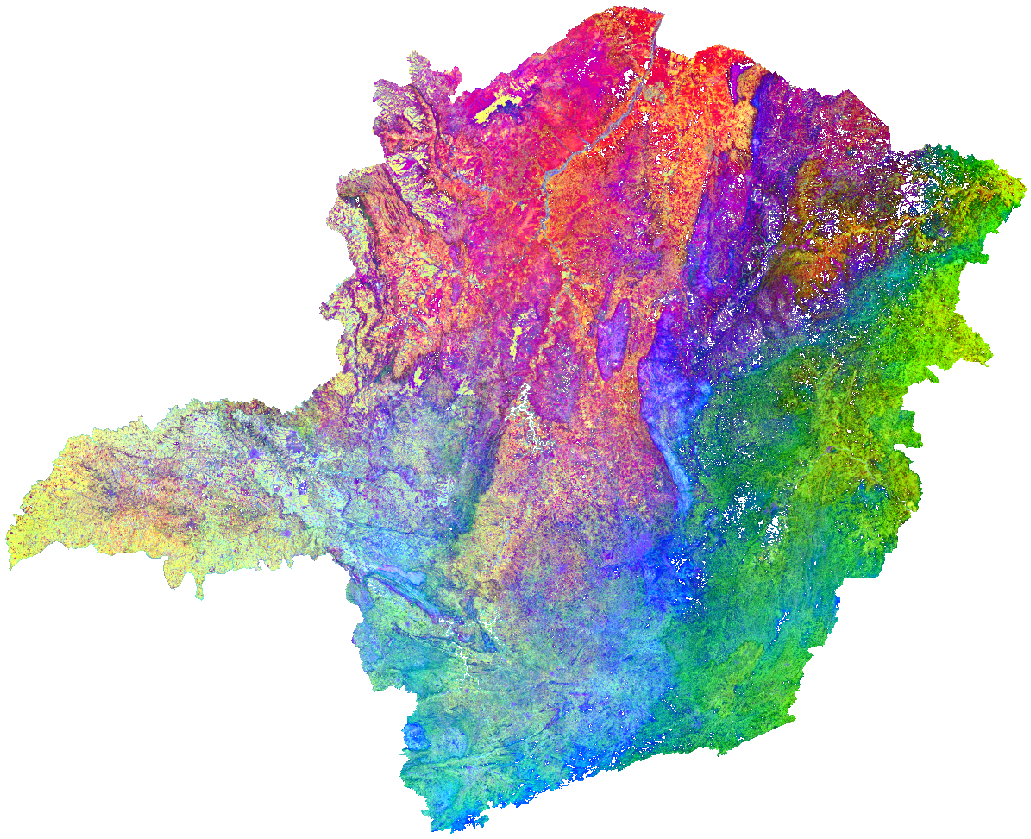
\includegraphics[height=0.78\paperheight]{hero_gsed.png}};
\end{tikzpicture}
\vfill
\begin{minipage}{0.6\textwidth}
  {\color{blue!25!white}\small Geographic Information Systems \ $\cdot$ \ Term Project \ $\cdot$ \ Mid-term Review}\\[14pt]
  {\color{white}\LARGE\bfseries Satellites, Night Lights and Words:}\\[6pt]
  {\color{white}\large\bfseries Estimating Municipal GDP from}\\[3pt]
  {\color{white}\large\bfseries Satellite Embeddings}\\[12pt]
  {\color{kgpgold}\rule{0.62\textwidth}{1.6pt}}\\[12pt]
  {\color{white}\normalsize\textbf{Hemant}\ \ (22CS30029)}\\[7pt]
  {\color{blue!25!white}\footnotesize Study area: Minas Gerais, Brazil \ $\cdot$ \ \nMunis{} municipalities \ $\cdot$ \ 1\,km grid}\\[2pt]
  {\color{blue!25!white}\footnotesize \texttt{github.com/chadsaras/GIS\_Project}}
\end{minipage}
\vfill
\end{frame}
}

%----------------------------- 2. PROBLEM ------------------------------
\begin{frame}{Problem Statement}
\begin{columns}[T,onlytextwidth]
\begin{column}{0.47\textwidth}
\begin{block}{Why Estimate GDP from Space?}
\footnotesize
\begin{itemize}\itemsep2pt
  \item Sub-national GDP is published \textbf{late}, often \textbf{estimated} from partial data,
        or \textbf{missing} in countries with weak statistical systems.
  \item Satellites observe every place, every year, with the same sensor --- an
        \textbf{independent, consistent} signal of economic activity.
  \item Inside one Brazilian state, GDP per capita already spans a \textbf{50$\times$} range
        (map): a hard, realistic test.
\end{itemize}
\end{block}
\vspace{7pt}
\begin{exampleblock}{Our Goal}
\small
Estimate 2022 GDP per capita for each of the \textbf{\nMunis{} municipalities} of Minas Gerais from
\textbf{free satellite data} --- and measure \textbf{honestly} how well it works.
\end{exampleblock}
\end{column}
\begin{column}{0.5\textwidth}
\centering
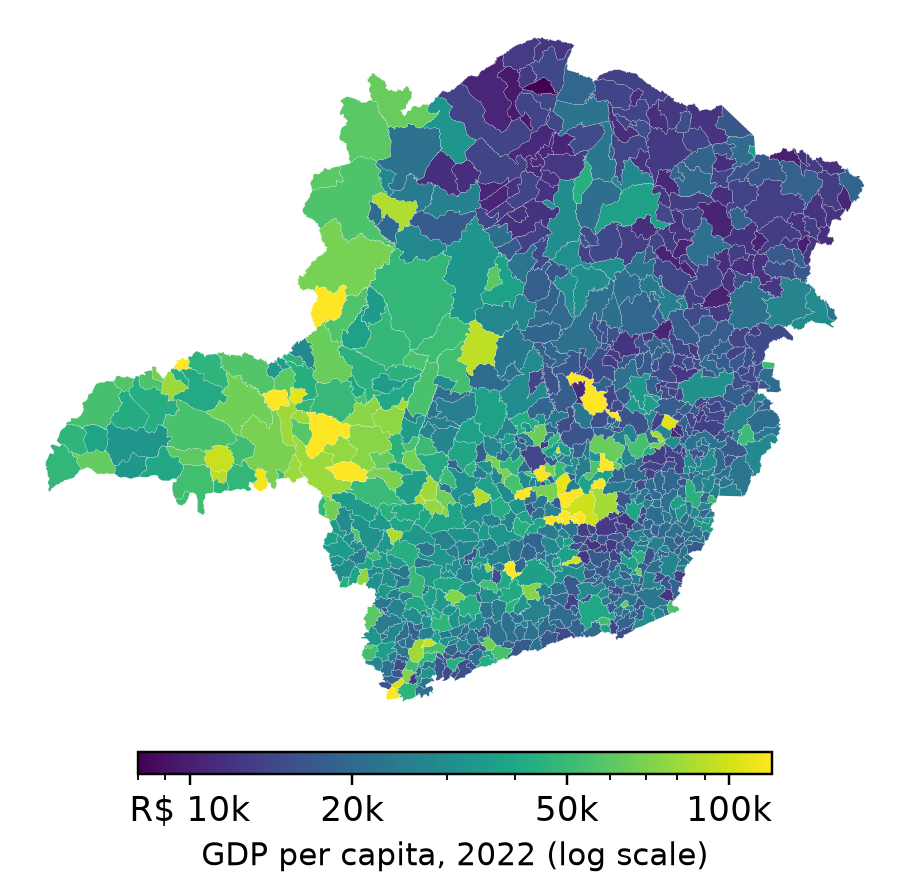
\includegraphics[height=5.6cm]{map_gdp.png}\\[-2pt]
{\scriptsize\color{mdlgrey}Official GDP per capita, 2022 (IBGE)}
\end{column}
\end{columns}
\end{frame}

%----------------------------- 3. TWO PAPERS ---------------------------
\begin{frame}{Building on Two Papers}
\headline{Two complementary ideas --- never combined, never tested at municipal level}
\begin{columns}[T,onlytextwidth]
\begin{column}{0.47\textwidth}
\begin{block}{UrbanCLIP \ {\normalfont\footnotesize(Yan et al., WWW 2024)}}
\footnotesize
A language model writes a \textbf{caption for each satellite tile}; images and captions are
aligned contrastively.\\[2pt]
{\color{kgpred}GDP gain only \textbf{+0.5\%} R\textsuperscript{2}; random split leaks neighbours; captions checked by hand.}
\end{block}
\vspace{6pt}
\begin{block}{Satellite Embeddings \ {\normalfont\footnotesize(Yue, Zhao \& Hu, 2026)}}
\footnotesize
Google's \textbf{64-number embeddings}, \textbf{steered by night lights} towards economic meaning.\\[2pt]
{\color{kgpred}Beats night lights for GDP levels --- but only across \textbf{countries}; no text, no POI/roads.}
\end{block}
\end{column}
\begin{column}{0.47\textwidth}
\begin{alertblock}{Gaps We Address}
\footnotesize
\begin{enumerate}\itemsep1.5pt
  \item The two ideas were \textbf{never combined}: do text and steering help each other?
  \item Random splits \textbf{overstate} accuracy (near-identical neighbours).
  \item Hand-checked captions \textbf{do not scale}.
  \item Country level gives \textbf{few training examples}.
\end{enumerate}
\end{alertblock}
\vspace{6pt}
\begin{exampleblock}{\nov{This Project}}
\footnotesize
Both ideas in \textbf{one pipeline} \ $\cdot$ \ \textbf{\nMunis{} municipalities} \ $\cdot$ \
\textbf{spatial} cross-validation \ $\cdot$ \ ablations of every ingredient \ $\cdot$ \
\textbf{automatic} caption checks
\end{exampleblock}
\end{column}
\end{columns}
\end{frame}

%----------------------------- 4. APPROACH -----------------------------
\begin{frame}{Our Approach: Three Stages, From No Labels to Official GDP}
\headline{Supervision gets scarcer and more expensive at each stage}
\vspace{2pt}
\makebox[\textwidth][c]{\resizebox{0.93\paperwidth}{!}{% ======================================================================
%  Pipeline diagram for the "Our Approach" slide (same visual language as AskTheSensors architecture.tex).
%  grey = inputs / output   blue = learning stages   gold star = our own contribution
%  In the deck:  % ======================================================================
%  Pipeline diagram for the "Our Approach" slide (same visual language as AskTheSensors architecture.tex).
%  grey = inputs / output   blue = learning stages   gold star = our own contribution
%  In the deck:  % ======================================================================
%  Pipeline diagram for the "Our Approach" slide (same visual language as AskTheSensors architecture.tex).
%  grey = inputs / output   blue = learning stages   gold star = our own contribution
%  In the deck:  \input{figures/pipeline.tex}
% ======================================================================
\definecolor{archblue}{HTML}{2F6FD6}
\definecolor{archbluebg}{HTML}{E3ECFB}
\definecolor{archgrey}{HTML}{6B7280}
\definecolor{archgreybg}{HTML}{F3F4F6}

\begin{tikzpicture}[
  >={Stealth[length=2.4mm,width=2mm]},
  box/.style={draw, rounded corners=3pt, line width=0.8pt, align=center,
              font=\sffamily\fontsize{7}{8.4}\selectfont, inner sep=4pt, minimum height=1.45cm},
  io/.style={box, draw=archgrey, fill=archgreybg, text width=2.7cm, minimum height=1.15cm},
  stage/.style={box, draw=archblue, fill=archbluebg, text width=3.0cm},
  flow/.style={->, line width=1pt, draw=kgpink!75},
  feed/.style={->, line width=0.8pt, draw=archgrey},
  badge/.style={circle, fill=kgpnavy, text=white, font=\sffamily\bfseries\fontsize{7}{8}\selectfont,
                inner sep=0pt, minimum size=4.4mm},
  lab/.style={font=\sffamily\bfseries\fontsize{6.5}{7.8}\selectfont, text=white, rounded corners=1.5pt,
              inner xsep=2.5pt, inner ysep=1.2pt},
  swatch/.style={minimum width=3.2mm, minimum height=2.5mm, inner sep=0pt, rounded corners=1pt, line width=0.7pt},
  note/.style={font=\sffamily\fontsize{7}{8.4}\selectfont, anchor=west},
]
\newcommand{\pbt}[1]{{\fontsize{9}{10.8}\selectfont\bfseries #1}\\[2pt]}

% ------------------------------ learning stages -------------------------------
\node[stage] (A) {\pbt{Image--text alignment}GSED and caption vectors\\pulled together (contrastive)};
\node[stage, right=0.75cm of A] (B) {\pbt{Night-light steering}predict each cell's lights;\\keep the 32-number layer};
\node[stage, right=0.75cm of B] (C) {\pbt{Municipal GDP}add up all cells of a\\municipality, then predict};
\node[io, right=0.6cm of C, text width=2.1cm, draw=kgpnavy, fill=kgpblue] (Y)
  {\pbt{log GDP}\textbf{per capita}\\853 municipalities};
\draw[flow] (A) -- (B); \draw[flow] (B) -- (C); \draw[flow] (C) -- (Y);

% supervision labels under each stage
\node[lab, fill=kgpgreen, below=3pt of A] {NO LABELS};
\node[lab, fill=kgpgold, below=3pt of B] {CHEAP PROXY LABEL};
\node[lab, fill=kgpred, below=3pt of C] {REAL LABEL};

% ----------------------------------- inputs -----------------------------------
\node[io, left=0.75cm of A] (g) {\pbt{Satellite\\embeddings}64 numbers per\\1\,km cell (GSED)};
\node[io, above=0.8cm of A, text width=3.3cm] (t) {\pbt{Captions + facts}VLM text, checked against\\land cover, roads, buildings};
\node[io, above=0.8cm of B] (n) {\pbt{Night lights}VIIRS 2022};
\node[io, above=0.8cm of C] (y) {\pbt{Official GDP}IBGE 2022};
\draw[flow] (g) -- (A);
\draw[feed] (t) -- (A); \draw[feed] (n) -- (B); \draw[feed] (y) -- (C);

% panel: everything retrained per spatial fold
\begin{scope}[on background layer]
  \node[draw=kgpnavy!45, fill=kgpblue!45, rounded corners=5pt, line width=0.6pt,
        inner xsep=8pt, inner ysep=13pt, fit=(A)(B)(C)] (panel) {};
\end{scope}
\node[anchor=south east, font=\sffamily\fontsize{6.5}{7.8}\selectfont, text=kgpnavy] at ($(panel.south east)+(-0.12,0.06)$)
  {all stages retrained per fold};

% badges and stars
\node[badge] (b1) at (A.north west) {1};
\node[badge] (b2) at (B.north west) {2};
\node[badge] (b3) at (C.north west) {3};
\node[text=kgpgold, anchor=west, inner sep=1pt] at (t.north west) {$\bigstar$};
\node[text=kgpgold, inner sep=1pt, fill=white, circle] at ($(A.east)!0.5!(B.west)+(0,0.32)$) {$\bigstar$};
\node[text=kgpgold, anchor=west, inner sep=1pt] at ($(panel.south west)+(0.1,0.12)$) {$\bigstar$};

% ----------------------------------- legend -----------------------------------
\node[swatch, draw=archgrey, fill=archgreybg, anchor=west] (lg1) at ($(g.west |- panel.south)+(0,-0.42)$) {};
\node[note] (lt1) at (lg1.east) {input / output};
\node[swatch, draw=archblue, fill=archbluebg, right=0.5cm of lt1] (lg2) {};
\node[note] (lt2) at (lg2.east) {learning stage (small networks)};
\node[text=kgpgold, right=0.5cm of lt2, inner sep=0pt] (lg3) {$\bigstar$};
\node[note] at (lg3.east) {our contribution: automatic caption checks, combining A with B, spatial testing};
\end{tikzpicture}

% ======================================================================
\definecolor{archblue}{HTML}{2F6FD6}
\definecolor{archbluebg}{HTML}{E3ECFB}
\definecolor{archgrey}{HTML}{6B7280}
\definecolor{archgreybg}{HTML}{F3F4F6}

\begin{tikzpicture}[
  >={Stealth[length=2.4mm,width=2mm]},
  box/.style={draw, rounded corners=3pt, line width=0.8pt, align=center,
              font=\sffamily\fontsize{7}{8.4}\selectfont, inner sep=4pt, minimum height=1.45cm},
  io/.style={box, draw=archgrey, fill=archgreybg, text width=2.7cm, minimum height=1.15cm},
  stage/.style={box, draw=archblue, fill=archbluebg, text width=3.0cm},
  flow/.style={->, line width=1pt, draw=kgpink!75},
  feed/.style={->, line width=0.8pt, draw=archgrey},
  badge/.style={circle, fill=kgpnavy, text=white, font=\sffamily\bfseries\fontsize{7}{8}\selectfont,
                inner sep=0pt, minimum size=4.4mm},
  lab/.style={font=\sffamily\bfseries\fontsize{6.5}{7.8}\selectfont, text=white, rounded corners=1.5pt,
              inner xsep=2.5pt, inner ysep=1.2pt},
  swatch/.style={minimum width=3.2mm, minimum height=2.5mm, inner sep=0pt, rounded corners=1pt, line width=0.7pt},
  note/.style={font=\sffamily\fontsize{7}{8.4}\selectfont, anchor=west},
]
\newcommand{\pbt}[1]{{\fontsize{9}{10.8}\selectfont\bfseries #1}\\[2pt]}

% ------------------------------ learning stages -------------------------------
\node[stage] (A) {\pbt{Image--text alignment}GSED and caption vectors\\pulled together (contrastive)};
\node[stage, right=0.75cm of A] (B) {\pbt{Night-light steering}predict each cell's lights;\\keep the 32-number layer};
\node[stage, right=0.75cm of B] (C) {\pbt{Municipal GDP}add up all cells of a\\municipality, then predict};
\node[io, right=0.6cm of C, text width=2.1cm, draw=kgpnavy, fill=kgpblue] (Y)
  {\pbt{log GDP}\textbf{per capita}\\853 municipalities};
\draw[flow] (A) -- (B); \draw[flow] (B) -- (C); \draw[flow] (C) -- (Y);

% supervision labels under each stage
\node[lab, fill=kgpgreen, below=3pt of A] {NO LABELS};
\node[lab, fill=kgpgold, below=3pt of B] {CHEAP PROXY LABEL};
\node[lab, fill=kgpred, below=3pt of C] {REAL LABEL};

% ----------------------------------- inputs -----------------------------------
\node[io, left=0.75cm of A] (g) {\pbt{Satellite\\embeddings}64 numbers per\\1\,km cell (GSED)};
\node[io, above=0.8cm of A, text width=3.3cm] (t) {\pbt{Captions + facts}VLM text, checked against\\land cover, roads, buildings};
\node[io, above=0.8cm of B] (n) {\pbt{Night lights}VIIRS 2022};
\node[io, above=0.8cm of C] (y) {\pbt{Official GDP}IBGE 2022};
\draw[flow] (g) -- (A);
\draw[feed] (t) -- (A); \draw[feed] (n) -- (B); \draw[feed] (y) -- (C);

% panel: everything retrained per spatial fold
\begin{scope}[on background layer]
  \node[draw=kgpnavy!45, fill=kgpblue!45, rounded corners=5pt, line width=0.6pt,
        inner xsep=8pt, inner ysep=13pt, fit=(A)(B)(C)] (panel) {};
\end{scope}
\node[anchor=south east, font=\sffamily\fontsize{6.5}{7.8}\selectfont, text=kgpnavy] at ($(panel.south east)+(-0.12,0.06)$)
  {all stages retrained per fold};

% badges and stars
\node[badge] (b1) at (A.north west) {1};
\node[badge] (b2) at (B.north west) {2};
\node[badge] (b3) at (C.north west) {3};
\node[text=kgpgold, anchor=west, inner sep=1pt] at (t.north west) {$\bigstar$};
\node[text=kgpgold, inner sep=1pt, fill=white, circle] at ($(A.east)!0.5!(B.west)+(0,0.32)$) {$\bigstar$};
\node[text=kgpgold, anchor=west, inner sep=1pt] at ($(panel.south west)+(0.1,0.12)$) {$\bigstar$};

% ----------------------------------- legend -----------------------------------
\node[swatch, draw=archgrey, fill=archgreybg, anchor=west] (lg1) at ($(g.west |- panel.south)+(0,-0.42)$) {};
\node[note] (lt1) at (lg1.east) {input / output};
\node[swatch, draw=archblue, fill=archbluebg, right=0.5cm of lt1] (lg2) {};
\node[note] (lt2) at (lg2.east) {learning stage (small networks)};
\node[text=kgpgold, right=0.5cm of lt2, inner sep=0pt] (lg3) {$\bigstar$};
\node[note] at (lg3.east) {our contribution: automatic caption checks, combining A with B, spatial testing};
\end{tikzpicture}

% ======================================================================
\definecolor{archblue}{HTML}{2F6FD6}
\definecolor{archbluebg}{HTML}{E3ECFB}
\definecolor{archgrey}{HTML}{6B7280}
\definecolor{archgreybg}{HTML}{F3F4F6}

\begin{tikzpicture}[
  >={Stealth[length=2.4mm,width=2mm]},
  box/.style={draw, rounded corners=3pt, line width=0.8pt, align=center,
              font=\sffamily\fontsize{7}{8.4}\selectfont, inner sep=4pt, minimum height=1.45cm},
  io/.style={box, draw=archgrey, fill=archgreybg, text width=2.7cm, minimum height=1.15cm},
  stage/.style={box, draw=archblue, fill=archbluebg, text width=3.0cm},
  flow/.style={->, line width=1pt, draw=kgpink!75},
  feed/.style={->, line width=0.8pt, draw=archgrey},
  badge/.style={circle, fill=kgpnavy, text=white, font=\sffamily\bfseries\fontsize{7}{8}\selectfont,
                inner sep=0pt, minimum size=4.4mm},
  lab/.style={font=\sffamily\bfseries\fontsize{6.5}{7.8}\selectfont, text=white, rounded corners=1.5pt,
              inner xsep=2.5pt, inner ysep=1.2pt},
  swatch/.style={minimum width=3.2mm, minimum height=2.5mm, inner sep=0pt, rounded corners=1pt, line width=0.7pt},
  note/.style={font=\sffamily\fontsize{7}{8.4}\selectfont, anchor=west},
]
\newcommand{\pbt}[1]{{\fontsize{9}{10.8}\selectfont\bfseries #1}\\[2pt]}

% ------------------------------ learning stages -------------------------------
\node[stage] (A) {\pbt{Image--text alignment}GSED and caption vectors\\pulled together (contrastive)};
\node[stage, right=0.75cm of A] (B) {\pbt{Night-light steering}predict each cell's lights;\\keep the 32-number layer};
\node[stage, right=0.75cm of B] (C) {\pbt{Municipal GDP}add up all cells of a\\municipality, then predict};
\node[io, right=0.6cm of C, text width=2.1cm, draw=kgpnavy, fill=kgpblue] (Y)
  {\pbt{log GDP}\textbf{per capita}\\853 municipalities};
\draw[flow] (A) -- (B); \draw[flow] (B) -- (C); \draw[flow] (C) -- (Y);

% supervision labels under each stage
\node[lab, fill=kgpgreen, below=3pt of A] {NO LABELS};
\node[lab, fill=kgpgold, below=3pt of B] {CHEAP PROXY LABEL};
\node[lab, fill=kgpred, below=3pt of C] {REAL LABEL};

% ----------------------------------- inputs -----------------------------------
\node[io, left=0.75cm of A] (g) {\pbt{Satellite\\embeddings}64 numbers per\\1\,km cell (GSED)};
\node[io, above=0.8cm of A, text width=3.3cm] (t) {\pbt{Captions + facts}VLM text, checked against\\land cover, roads, buildings};
\node[io, above=0.8cm of B] (n) {\pbt{Night lights}VIIRS 2022};
\node[io, above=0.8cm of C] (y) {\pbt{Official GDP}IBGE 2022};
\draw[flow] (g) -- (A);
\draw[feed] (t) -- (A); \draw[feed] (n) -- (B); \draw[feed] (y) -- (C);

% panel: everything retrained per spatial fold
\begin{scope}[on background layer]
  \node[draw=kgpnavy!45, fill=kgpblue!45, rounded corners=5pt, line width=0.6pt,
        inner xsep=8pt, inner ysep=13pt, fit=(A)(B)(C)] (panel) {};
\end{scope}
\node[anchor=south east, font=\sffamily\fontsize{6.5}{7.8}\selectfont, text=kgpnavy] at ($(panel.south east)+(-0.12,0.06)$)
  {all stages retrained per fold};

% badges and stars
\node[badge] (b1) at (A.north west) {1};
\node[badge] (b2) at (B.north west) {2};
\node[badge] (b3) at (C.north west) {3};
\node[text=kgpgold, anchor=west, inner sep=1pt] at (t.north west) {$\bigstar$};
\node[text=kgpgold, inner sep=1pt, fill=white, circle] at ($(A.east)!0.5!(B.west)+(0,0.32)$) {$\bigstar$};
\node[text=kgpgold, anchor=west, inner sep=1pt] at ($(panel.south west)+(0.1,0.12)$) {$\bigstar$};

% ----------------------------------- legend -----------------------------------
\node[swatch, draw=archgrey, fill=archgreybg, anchor=west] (lg1) at ($(g.west |- panel.south)+(0,-0.42)$) {};
\node[note] (lt1) at (lg1.east) {input / output};
\node[swatch, draw=archblue, fill=archbluebg, right=0.5cm of lt1] (lg2) {};
\node[note] (lt2) at (lg2.east) {learning stage (small networks)};
\node[text=kgpgold, right=0.5cm of lt2, inner sep=0pt] (lg3) {$\bigstar$};
\node[note] at (lg3.east) {our contribution: automatic caption checks, combining A with B, spatial testing};
\end{tikzpicture}
}}
\vspace{4pt}
\source{Captions are needed only for training: at prediction time each cell uses its embedding alone.
Switching stages off gives the ablations (variants V3--V9).}
\end{frame}

%----------------------------- 5. DATA ---------------------------------
\begin{frame}{Data: Six Free Layers on One 1\,km Grid}
\headline{Every layer averaged onto the same 1\,km cells; the GDP target is official statistics, not night lights}
\begin{columns}[c,onlytextwidth]
\begin{column}{0.64\textwidth}
\centering
\thumb{thumb_gsed.png}{Satellite embeddings}{Google GSED, 10\,m $\rightarrow$ 1\,km}\hfill
\thumb{thumb_ntl.png}{Night lights}{VIIRS 2022}\hfill
\thumb{thumb_built.png}{Built-up land}{ESA WorldCover}\\[6pt]
\thumb{thumb_roads.png}{Roads and POIs}{OpenStreetMap}\hfill
\thumb{thumb_buildings.png}{Building footprints}{Microsoft + OSM}\hfill
\thumb{thumb_gdp.png}{GDP and population}{IBGE 2022 (target)}
\end{column}
\begin{column}{0.34\textwidth}
\centering
\ctile[1.95cm]{kgpnavy}{kgpblue}{\nMunis}{municipalities}\hspace{2pt}%
\ctile[1.95cm]{kgpnavy}{kgpblue}{\nCells}{1\,km cells}\\[5pt]
\ctile[1.95cm]{kgpgreen}{kgpgreenbg}{10k}{captioned tiles}\hspace{2pt}%
\ctile[1.95cm]{kgpgold}{kgpgold!10}{\nBuildings}{building footprints}
\end{column}
\end{columns}
\end{frame}

%----------------------------- 6. CAPTIONS (INNOVATION 1) --------------
\begin{frame}{\nov{Innovation 1: Captions Checked Against the Data}}
\headline{A vision--language model describes each tile; claims the map data contradicts are removed automatically}
\begin{columns}[T,onlytextwidth]
\begin{column}{0.31\textwidth}
\centering
{\scriptsize\bfseries\color{kgpnavy}A real tile from our sample}\\[2pt]
\begin{tikzpicture}
  \node[inner sep=0] (im) {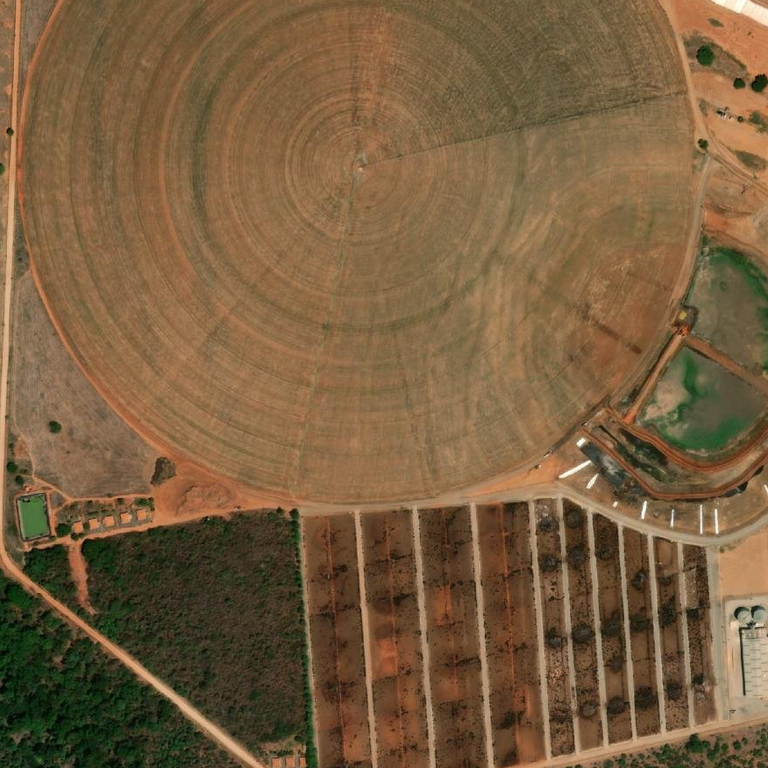
\includegraphics[width=\linewidth]{caption_tile.png}};
  \begin{scope}[x={($(im.south east)-(im.south west)$)},y={($(im.north west)-(im.south west)$)},shift={(im.south west)}]
    \draw[kgpred,line width=1.3pt,dashed] (0.43,0.64) ellipse (0.36 and 0.33);
    \node[anchor=south west,font=\scriptsize\bfseries,fill=white,fill opacity=0.9,text opacity=1,text=kgpred,inner sep=2pt]
      at (0.02,0.02) {centre-pivot irrigation, not a mine};
  \end{scope}
\end{tikzpicture}\\[1pt]
{\tiny\color{mdlgrey}Esri World Imagery, \textasciitilde1\,m per pixel}
\end{column}
\begin{column}{0.4\textwidth}
\fcolorbox{kgpnavy!60}{white}{\parbox{0.95\linewidth}{\raggedright
{\scriptsize\bfseries\color{kgpnavy}Qwen2.5-VL-7B caption, after the checks}
\begin{itemize}\setlength{\itemsep}{1pt}\scriptsize
\dropped{The satellite image shows a large circular area with concentric rings, likely a mine pit, surrounded by a grid of smaller rectangular plots of farmland.}{unsupported industry claim}
\keep{Roads crisscross the area, connecting the plots and the perimeter.}
\keep{Vegetation is sparse, mostly along the edges and in some patches within the farmland.}
\keep{A small body of water, possibly a pond, is visible near the farmland.}
\keep{No buildings or industrial structures are evident, suggesting minimal built-up area.}
\dropped{The overall scene appears to be an agricultural landscape with a focus on farming and possibly mining operations.}{filler}

\end{itemize}}}
\end{column}
\begin{column}{0.26\textwidth}
{\scriptsize\bfseries\color{kgpnavy}What the checks removed}\\[2pt]
\scriptsize
\renewcommand{\arraystretch}{1.1}
\begin{tabular}{@{}l r@{}}
\toprule
Reason & Sentences \\
\midrule
Filler & \nDropFiller \\
Industry claim & \nDropIndustry \\
Building claim & \nDropBuilding \\
Water claim & \nDropWater \\
Road claim & \nDropRoad \\
Farmland claim & \nDropFarm \\
\midrule
\textbf{Kept} & \ev{\nKept} \\
\bottomrule
\end{tabular}\\[4pt]
{\tiny\color{mdlgrey}of \nSentences{} sentences in \nCaptions{} captions; image--text matching removes \nClipDropped{} more captions}
\end{column}
\end{columns}
\vspace{4pt}
\source{Checks use ESA land cover, OSM roads and Microsoft + OSM building footprints. A blind hand audit of 300 captions is in progress.}
\end{frame}

%----------------------------- 7. EVALUATION (INNOVATION 2) ------------
\begin{frame}{\nov{Innovation 2: An Honest Test}}
\headline{Whole regions are held out, so no test municipality has a look-alike neighbour in training}
\begin{columns}[c,onlytextwidth]
\begin{column}{0.46\textwidth}
\centering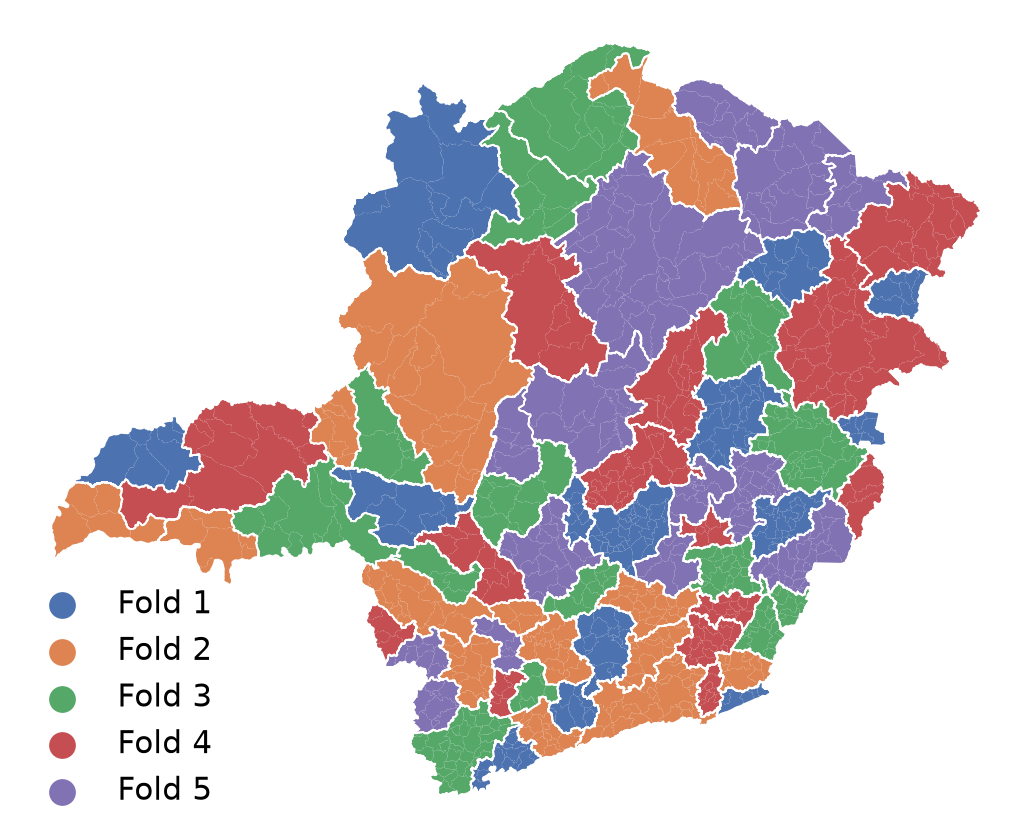
\includegraphics[height=5.1cm]{map_folds.png}
\end{column}
\begin{column}{0.5\textwidth}
\begin{block}{How We Split}
\footnotesize
\begin{enumerate}\itemsep1.5pt
  \item \textbf{70 official regions} of neighbouring municipalities $\rightarrow$ 5 balanced folds.
  \item Each round: 3 folds train, 1 validates, \textbf{1 is tested}; \textbf{all stages are retrained}.
  \item Every municipality is tested \textbf{exactly once}, by a model that never saw its region.
\end{enumerate}
\end{block}
\vspace{3pt}
\begin{alertblock}{Why It Matters}
\footnotesize
UrbanCLIP split tiles \textbf{at random} (60/20/20): near-identical neighbours land in both
training and test, inflating the scores.
\end{alertblock}
\vspace{3pt}
\begin{exampleblock}{Fair Comparisons}
\footnotesize
Same folds for every model; differences tested with a \textbf{block bootstrap} over regions (95\% intervals).
\end{exampleblock}
\end{column}
\end{columns}
\end{frame}

%----------------------------- 8. RESULTS ------------------------------
\begin{frame}{Headline Results: The Hybrid Explains Half of GDP Variation}
\headline{\nMunis{} municipalities \ $\cdot$ \ 5 spatial folds \ $\cdot$ \ every municipality tested once, in a region never seen}
\begin{columns}[c,onlytextwidth]
\begin{column}{0.63\textwidth}
\centering
\resizebox{\linewidth}{!}{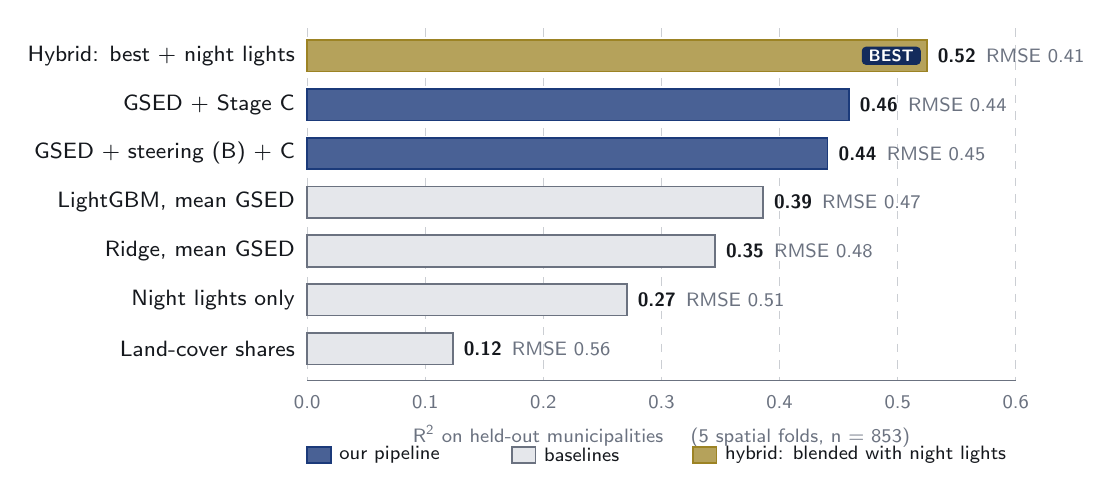
\begin{tikzpicture}[x=1cm,y=1cm,
  mname/.style={font=\sffamily\fontsize{8}{9.6}\selectfont,text=kgpink,anchor=east,inner sep=0pt},
  val/.style={font=\sffamily\fontsize{7.5}{9}\selectfont,text=kgpink,anchor=west,inner xsep=1.5pt},
  tick/.style={font=\sffamily\fontsize{7}{8.4}\selectfont,text=mdlgrey,anchor=north},
  tag/.style={font=\sffamily\bfseries\fontsize{6.5}{7.8}\selectfont,text=white,rounded corners=1.5pt,inner xsep=2.5pt,inner ysep=1.2pt,anchor=east}]
\draw[mdlgrey!35,line width=0.4pt,dashed] (0.00,0.35) -- (0.00,-4.12);
\node[tick] at (0.00,-4.20) {0.0};
\draw[mdlgrey!35,line width=0.4pt,dashed] (1.50,0.35) -- (1.50,-4.12);
\node[tick] at (1.50,-4.20) {0.1};
\draw[mdlgrey!35,line width=0.4pt,dashed] (3.00,0.35) -- (3.00,-4.12);
\node[tick] at (3.00,-4.20) {0.2};
\draw[mdlgrey!35,line width=0.4pt,dashed] (4.50,0.35) -- (4.50,-4.12);
\node[tick] at (4.50,-4.20) {0.3};
\draw[mdlgrey!35,line width=0.4pt,dashed] (6.00,0.35) -- (6.00,-4.12);
\node[tick] at (6.00,-4.20) {0.4};
\draw[mdlgrey!35,line width=0.4pt,dashed] (7.50,0.35) -- (7.50,-4.12);
\node[tick] at (7.50,-4.20) {0.5};
\draw[mdlgrey!35,line width=0.4pt,dashed] (9.00,0.35) -- (9.00,-4.12);
\node[tick] at (9.00,-4.20) {0.6};
\draw[mdlgrey,line width=0.5pt] (0,-4.12) -- (9.00,-4.12);
\node[tick] at (4.50,-4.57) {R\textsuperscript{2} on held-out municipalities \quad (5 spatial folds, n = 853)};
\node[mname] at (-0.15,-0.00) {Hybrid: best + night lights};
\path[draw=kgpgold,fill=kgpgold!75,line width=0.6pt] (0,-0.20) rectangle (7.87,0.20);
\node[val] at (7.95,-0.00) {\textbf{0.52}\enspace\textcolor{mdlgrey}{RMSE 0.41}};
\node[tag,fill=kgpnavydark] at (7.80,-0.00) {BEST};
\node[mname] at (-0.15,-0.62) {GSED + Stage C};
\path[draw=kgpnavy,fill=kgpnavy!80,line width=0.6pt] (0,-0.82) rectangle (6.88,-0.42);
\node[val] at (6.96,-0.62) {\textbf{0.46}\enspace\textcolor{mdlgrey}{RMSE 0.44}};
\node[mname] at (-0.15,-1.24) {GSED + steering (B) + C};
\path[draw=kgpnavy,fill=kgpnavy!80,line width=0.6pt] (0,-1.44) rectangle (6.61,-1.04);
\node[val] at (6.69,-1.24) {\textbf{0.44}\enspace\textcolor{mdlgrey}{RMSE 0.45}};
\node[mname] at (-0.15,-1.86) {LightGBM, mean GSED};
\path[draw=mdlgrey,fill=mdlgreybg,line width=0.6pt] (0,-2.06) rectangle (5.79,-1.66);
\node[val] at (5.87,-1.86) {\textbf{0.39}\enspace\textcolor{mdlgrey}{RMSE 0.47}};
\node[mname] at (-0.15,-2.48) {Ridge, mean GSED};
\path[draw=mdlgrey,fill=mdlgreybg,line width=0.6pt] (0,-2.68) rectangle (5.18,-2.28);
\node[val] at (5.26,-2.48) {\textbf{0.35}\enspace\textcolor{mdlgrey}{RMSE 0.48}};
\node[mname] at (-0.15,-3.10) {Night lights only};
\path[draw=mdlgrey,fill=mdlgreybg,line width=0.6pt] (0,-3.30) rectangle (4.06,-2.90);
\node[val] at (4.14,-3.10) {\textbf{0.27}\enspace\textcolor{mdlgrey}{RMSE 0.51}};
\node[mname] at (-0.15,-3.72) {Land-cover shares};
\path[draw=mdlgrey,fill=mdlgreybg,line width=0.6pt] (0,-3.92) rectangle (1.85,-3.52);
\node[val] at (1.93,-3.72) {\textbf{0.12}\enspace\textcolor{mdlgrey}{RMSE 0.56}};
\path[draw=kgpnavy,fill=kgpnavy!80,line width=0.6pt] (0,-5.17) rectangle (0.3,-4.97);
\node[val] at (0.35,-5.07) {our pipeline};
\path[draw=mdlgrey,fill=mdlgreybg,line width=0.6pt] (2.6,-5.17) rectangle (2.9,-4.97);
\node[val] at (2.95,-5.07) {baselines};
\path[draw=kgpgold,fill=kgpgold!75,line width=0.6pt] (4.9,-5.17) rectangle (5.2,-4.97);
\node[val] at (5.25,-5.07) {hybrid: blended with night lights};
\end{tikzpicture}
}
\end{column}
\begin{column}{0.35\textwidth}
\centering

\begin{tikzpicture}
  \node[draw=kgpgold, fill=kgpgold!10, rounded corners=4pt, line width=0.9pt, align=center,
        text width=0.9\linewidth, inner sep=6pt]
    {{\fontsize{26}{28}\selectfont\bfseries\color{kgpgold}\nHybridR}\\[3pt]
     {\footnotesize\bfseries R\textsuperscript{2} of the hybrid model}\\[1pt]
     {\scriptsize RMSE \nHybridRMSE{} \ $\cdot$ \ night lights alone: R\textsuperscript{2} \nNtlR}};
\end{tikzpicture}\\[6pt]
\begin{block}{Research Questions So Far}
\scriptsize
\lchip{kgpslate}{RQ1 STEERING}\ \RQone\\[3pt]
\lchip{kgpgreen}{RQ4 HYBRID}\ \RQfour\\[3pt]
\lchip{kgpamber}{RQ2--3 TEXT, POI}\ text variants V5--V9 finishing now
\end{block}
\end{column}
\end{columns}
\vspace{2pt}
\source{Source: reports/tables/main\_results.csv, rq\_tests.csv. Hybrid = best model blended with the night-light benchmark (weight chosen on validation).}
\end{frame}

%----------------------------- 9. LESSONS ------------------------------
\begin{frame}{What We Learned: Calibration Mattered More Than Steering}
\headline{Fixing over-confident predictions improved error more than any new ingredient}
\begin{columns}[c,onlytextwidth]
\begin{column}{0.5\textwidth}
\centering
\resizebox{\linewidth}{!}{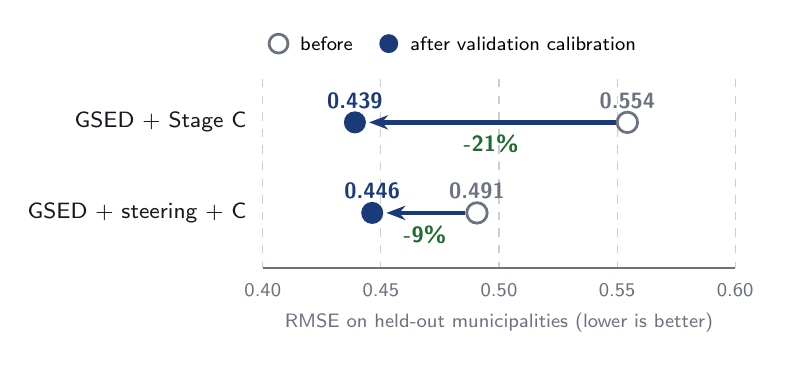
\begin{tikzpicture}[x=1cm,y=1cm,
  mname/.style={font=\sffamily\fontsize{8}{9.6}\selectfont,text=kgpink,anchor=east,inner sep=0pt},
  num/.style={font=\sffamily\bfseries\fontsize{8}{9.6}\selectfont,inner sep=1pt},
  tick/.style={font=\sffamily\fontsize{7}{8.4}\selectfont,text=mdlgrey,anchor=north}]
\draw[mdlgrey!35,line width=0.4pt,dashed] (0.00,0.55) -- (0.00,-1.85);
\node[tick] at (0.00,-1.93) {0.40};
\draw[mdlgrey!35,line width=0.4pt,dashed] (1.50,0.55) -- (1.50,-1.85);
\node[tick] at (1.50,-1.93) {0.45};
\draw[mdlgrey!35,line width=0.4pt,dashed] (3.00,0.55) -- (3.00,-1.85);
\node[tick] at (3.00,-1.93) {0.50};
\draw[mdlgrey!35,line width=0.4pt,dashed] (4.50,0.55) -- (4.50,-1.85);
\node[tick] at (4.50,-1.93) {0.55};
\draw[mdlgrey!35,line width=0.4pt,dashed] (6.00,0.55) -- (6.00,-1.85);
\node[tick] at (6.00,-1.93) {0.60};
\draw[mdlgrey,line width=0.5pt] (0,-1.85) -- (6.00,-1.85);
\node[tick] at (3.00,-2.3) {RMSE on held-out municipalities (lower is better)};
\node[mname] at (-0.2,-0.00) {GSED + Stage C};
\draw[-{Stealth[length=2.4mm]},kgpnavy,line width=1.6pt] (4.48,-0.00) -- (1.35,-0.00);
\node[circle,draw=mdlgrey,fill=white,line width=1pt,minimum size=2.6mm,inner sep=0pt] at (4.63,-0.00) {};
\node[circle,fill=kgpnavy,minimum size=2.8mm,inner sep=0pt] at (1.17,-0.00) {};
\node[num,text=mdlgrey,anchor=south] at (4.63,0.14) {0.554};
\node[num,text=kgpnavy,anchor=south] at (1.17,0.14) {0.439};
\node[num,text=kgpgreen,anchor=north] at (2.90,-0.12) {-21\%};
\node[mname] at (-0.2,-1.15) {GSED + steering + C};
\draw[-{Stealth[length=2.4mm]},kgpnavy,line width=1.6pt] (2.57,-1.15) -- (1.57,-1.15);
\node[circle,draw=mdlgrey,fill=white,line width=1pt,minimum size=2.6mm,inner sep=0pt] at (2.72,-1.15) {};
\node[circle,fill=kgpnavy,minimum size=2.8mm,inner sep=0pt] at (1.39,-1.15) {};
\node[num,text=mdlgrey,anchor=south] at (2.72,-1.01) {0.491};
\node[num,text=kgpnavy,anchor=south] at (1.39,-1.01) {0.446};
\node[num,text=kgpgreen,anchor=north] at (2.06,-1.27) {-9\%};
\node[circle,draw=mdlgrey,fill=white,line width=1pt,minimum size=2.4mm,inner sep=0pt] at (0.2,1.0) {};
\node[font=\sffamily\fontsize{7.5}{9}\selectfont,anchor=west] at (0.35,1.0) {before};
\node[circle,fill=kgpnavy,minimum size=2.4mm,inner sep=0pt] at (1.6,1.0) {};
\node[font=\sffamily\fontsize{7.5}{9}\selectfont,anchor=west] at (1.75,1.0) {after validation calibration};
\end{tikzpicture}
}
\end{column}
\begin{column}{0.47\textwidth}
\footnotesize
\begin{enumerate}\itemsep5pt
  \item \textbf{Predictions were over-spread.} Rich places came out too rich, poor too poor
        (slope 0.6). A straight-line correction fitted on \textbf{validation} cut error by \textbf{\textasciitilde20\%}.
  \item \textbf{Honest re-testing changes conclusions.} Night-light steering looked helpful before
        the fix; afterwards the gain \textbf{vanished}.
  \item \textbf{Captions need checking.} On featureless tiles the model invents mines, roads
        and farmland; the data checks remove most of it.
\end{enumerate}
\end{column}
\end{columns}
\vspace{6pt}
\source{Same models and folds before and after; the correction uses validation municipalities only.}
\end{frame}

%----------------------------- 10. PROGRESS ----------------------------
\begin{frame}{Progress and Next Steps}
\headline{About 80\% done --- the text experiments finish this week}
\begin{columns}[T,onlytextwidth]
\begin{column}{0.52\textwidth}
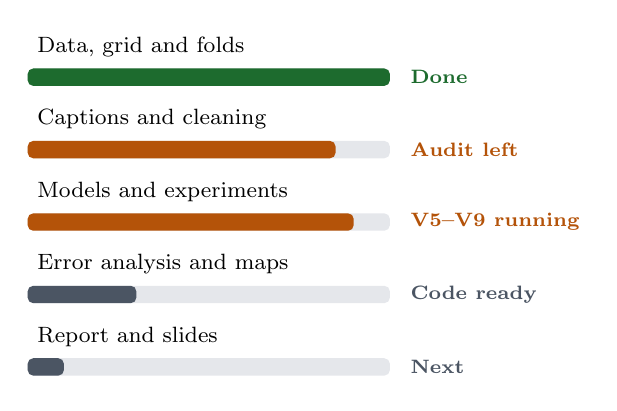
\begin{tikzpicture}[x=4.6cm,y=0.92cm]
  \foreach \lab/\pct/\fc/\st [count=\i] in {
      {Data, grid and folds}/1.00/kgpgreen/Done,
      Captions and cleaning/0.85/kgpamber/Audit left,
      Models and experiments/0.90/kgpamber/V5--V9 running,
      Error analysis and maps/0.30/kgpslate/Code ready,
      Report and slides/0.10/kgpslate/Next} {
    \node[anchor=west,font=\footnotesize] at (0,-\i+0.24) {\lab};
    \fill[mdlgreybg,rounded corners=2pt] (0,-\i-0.06) rectangle (1,-\i-0.3);
    \fill[\fc,rounded corners=2pt] (0,-\i-0.06) rectangle (\pct,-\i-0.3);
    \node[anchor=west,font=\scriptsize\bfseries,text=\fc] at (1.03,-\i-0.18) {\st};
  }
\end{tikzpicture}
\end{column}
\begin{column}{0.44\textwidth}
\scriptsize
\renewcommand{\arraystretch}{1.25}
\begin{tabular}{@{}L{0.62\linewidth}l@{}}
\toprule
\textbf{Research question} & \textbf{Status} \\
\midrule
RQ1 \ Night-light steering & \lchip{kgpgreen}{ANSWERED} \\
RQ2 \ Text (captions) & \lchip{kgpamber}{RUNNING} \\
RQ3 \ POIs and roads & \lchip{kgpamber}{RUNNING} \\
RQ4 \ Hybrid with night lights & \lchip{kgpgreen}{ANSWERED} \\
RQ5 \ Where it fails & \lchip{kgpslate}{NEXT} \\
\bottomrule
\end{tabular}
\vspace{8pt}
\begin{exampleblock}{Next}
\scriptsize
text results \ $\rightarrow$ \ caption audit \ $\rightarrow$ \ error analysis and 1\,km maps \ $\rightarrow$ \ report
\end{exampleblock}
\end{column}
\end{columns}
\end{frame}

%----------------------------- 11. SUMMARY -----------------------------
\begin{frame}{Summary}
\vspace{2pt}
\begin{center}
{\large\bfseries\color{kgpnavy}Free satellite embeddings, checked captions and night lights,\\[2pt]
tested honestly on \nMunis{} Brazilian municipalities.\par}
\end{center}
\vspace{6pt}
\begin{center}
\ctile{kgpgold}{kgpgold!10}{\nHybridR}{R\textsuperscript{2} of the hybrid\\on unseen regions}\hspace{0.28cm}%
\ctile{kgpnavy}{kgpblue}{\nNtlR}{R\textsuperscript{2} of night\\lights alone}\hspace{0.28cm}%
\ctile{kgpgreen}{kgpgreenbg}{\nKept}{caption sentences\\kept after checks}\hspace{0.28cm}%
\ctile{kgpgreen}{kgpgreenbg}{\nCalibGain}{error after\\calibration}
\end{center}
\vspace{4pt}
{\centering\footnotesize\color{kgpred}\textbf{Still open:} whether text and POIs add information (RQ2--3), and where the model fails (RQ5).\par}
\vspace{8pt}
{\centering{\Large\bfseries\color{kgpink}Questions?}\\[4pt]
{\footnotesize\color{kgpink!75}\texttt{github.com/chadsaras/GIS\_Project}}\par}
\end{frame}

%----------------------------- BACKUP ----------------------------------
\begin{frame}{Backup: Data Sources}
\scriptsize
\renewcommand{\arraystretch}{1.2}
\makebox[\textwidth][c]{%
\begin{tabular}{@{}L{0.2\textwidth}L{0.42\textwidth}L{0.33\textwidth}@{}}
\toprule
\textbf{Layer} & \textbf{Source} & \textbf{Use} \\
\midrule
Satellite embeddings & Google Satellite Embedding V1 (AlphaEarth), 2022 & image input, averaged 10\,m $\rightarrow$ 1\,km \\
Night lights & VIIRS DNB annual V2.2, 2022 & Stage B proxy label; night-light benchmark \\
Land cover & ESA WorldCover v200, 2021 & masking, fact sentences, caption checks \\
Roads, POIs & OpenStreetMap (Geofabrik, 2023-01-01) & features, fact sentences, caption checks \\
Buildings & Microsoft ML footprints + OSM & caption checks \\
Caption imagery & Esri World Imagery (ArcGIS Location Platform) & input to the vision--language model \\
GDP, population & IBGE municipal GDP 2022, Census 2022 & target: log GDP per capita \\
\bottomrule
\end{tabular}}
\end{frame}

\begin{frame}{Backup: Stage A Aligns Embeddings and Captions}
\headline{For a validation tile, how often is its own caption among the top $k$ of 256 candidates?}
\begin{columns}[c,onlytextwidth]
\begin{column}{0.5\textwidth}
\centering\resizebox{0.95\linewidth}{!}{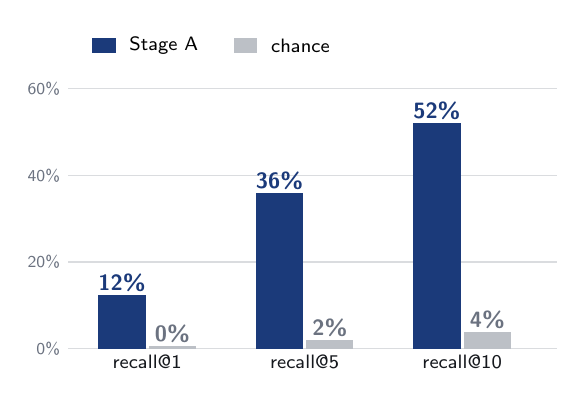
\begin{tikzpicture}[x=1cm,y=1cm,
  lbl/.style={font=\sffamily\fontsize{7.5}{9}\selectfont,text=kgpink,anchor=north,inner sep=0pt},
  num/.style={font=\sffamily\bfseries\fontsize{8}{9.6}\selectfont,anchor=south,inner sep=1pt},
  tick/.style={font=\sffamily\fontsize{6.5}{7.8}\selectfont,text=mdlgrey,anchor=east,inner sep=0pt}]
\draw[mdlgrey!25,line width=0.4pt] (0,0.00) -- (6.2,0.00);
\node[tick] at (-0.1,0.00) {0\%};
\draw[mdlgrey!25,line width=0.4pt] (0,1.10) -- (6.2,1.10);
\node[tick] at (-0.1,1.10) {20\%};
\draw[mdlgrey!25,line width=0.4pt] (0,2.20) -- (6.2,2.20);
\node[tick] at (-0.1,2.20) {40\%};
\draw[mdlgrey!25,line width=0.4pt] (0,3.30) -- (6.2,3.30);
\node[tick] at (-0.1,3.30) {60\%};
\fill[kgpnavy] (0.38,0) rectangle (0.98,0.68);
\node[num,text=kgpnavy] at (0.68,0.68) {12\%};
\fill[mdlgrey!45] (1.02,0) rectangle (1.62,0.03);
\node[num,text=mdlgrey] at (1.32,0.03) {0\%};
\node[lbl] at (1.00,-0.08) {recall@1};
\fill[kgpnavy] (2.38,0) rectangle (2.98,1.98);
\node[num,text=kgpnavy] at (2.68,1.98) {36\%};
\fill[mdlgrey!45] (3.02,0) rectangle (3.62,0.11);
\node[num,text=mdlgrey] at (3.32,0.11) {2\%};
\node[lbl] at (3.00,-0.08) {recall@5};
\fill[kgpnavy] (4.38,0) rectangle (4.98,2.87);
\node[num,text=kgpnavy] at (4.68,2.87) {52\%};
\fill[mdlgrey!45] (5.02,0) rectangle (5.62,0.21);
\node[num,text=mdlgrey] at (5.32,0.21) {4\%};
\node[lbl] at (5.00,-0.08) {recall@10};
\fill[kgpnavy] (0.3,3.75) rectangle (0.6,3.95); \node[font=\sffamily\fontsize{7.5}{9}\selectfont,anchor=west] at (0.65,3.85) {Stage A};
\fill[mdlgrey!45] (2.1,3.75) rectangle (2.4,3.95); \node[font=\sffamily\fontsize{7.5}{9}\selectfont,anchor=west] at (2.45,3.85) {chance};
\end{tikzpicture}
}
\end{column}
\begin{column}{0.46\textwidth}
\footnotesize
About \textbf{13$\times$ chance} at recall@10. Part of the alignment comes from the fact sentences;
variants \textbf{V8} (captions only) and \textbf{V9} (facts only) separate the two.
\end{column}
\end{columns}
\end{frame}

\begin{frame}{Backup: What the Captions Look Like}
\vspace{4pt}
\btile{backup_tile1.png}{\bcapnameA}{\bcapA}\hfill
\btile{backup_tile2.png}{\bcapnameB}{\bcapB}\hfill
\btile{backup_tile3.png}{\bcapnameC}{\bcapC}\hfill
\btile{backup_tile4.png}{\bcapnameD}{\bcapD}\par
\vspace{6pt}
\source{First sentence of each caption that passed the checks.}
\end{frame}

\end{document}
